
\begin{frame}\frametitle{A successful theory}
\scriptsize\centering

\begin{minipage}{.55\textwidth}\centering

\resizebox{1.\textwidth}{!}{\tiny
\begin{tabular}{c x{.12\textwidth} x{.12\textwidth} x{.12\textwidth} x{.12\textwidth}}\toprule
Fermions   & \multicolumn{2}{c}{Leptons}&\multicolumn{2}{c}{Quarks} \\ 
generation & $q=-1$ & $q=0$ &$q=\frac{2}{3}$ &$q=-\frac{1}{3}$ \\ \midrule
I & $e^{-}$ & $\nu_{e}$ & $u$ & $d$ \\
II & $\mu^{-}$ & $\nu_{\mu}$ & $c$ & $s$ \\
III & $\tau^{-}$ & $\nu_{\tau}$ & $t$ & $b$ \\ \midrule%\bottomrule\toprule
Force & Electromagnetic &\multicolumn{2}{c}{Weak}& Strong\\\midrule
Carrier boson & $\gamma$ & $W^{\pm}$ &$Z$ & $g$\\
spin & 1 & 1 &  1 & 1 \\
$q$ & 0 & $\pm$1 & 0 & 0\\ \midrule%\bottomrule\toprule
 \multicolumn{2}{c}{Higgs boson $H$}& \multicolumn{3}{c}{$q=0$, spin=0} \\
\bottomrule
\end{tabular}
}

\begin{pgfpicture}{0.0\textwidth}{0.0\textheight}{1.\textwidth}{.5\textwidth}

\begin{pgfscope}
%\pgfdeclareimage[interpolate=true,width=.75\textwidth]{wtop}{pics/W_vs_top}
\pgfdeclareimage[interpolate=true,width=.75\textwidth]{higgsatlas}{pics/HiggsComb_P0_2012July.png}%higgsatlas}
%\pgfputat{\pgfxy(.8,-0.2)}{\pgfbox[left,base]{\pgfuseimage{wtop}}}
 \pgfsetlinewidth{1.pt}
 \usebeamercolor[fg]{head/foot boxes}
\only<2>{
 \pgfrect[stroke]{\pgfxy(2,5.48)}{\pgfxy(1.7,0.57)}
 \begin{pgfrotateby}{\pgfdegree{30}}
 \pgfputat{\pgfxy(3.,4.3)}{\pgfbox[left,base]{\scriptsize\bf\begin{tabular}{c} ``who ordered\\ that??''\\\tiny [I.I.Rabi]\\\end{tabular}}}
 \end{pgfrotateby}
}
\only<3>{
 \pgfrect[stroke]{\pgfxy(4.6,5.75)}{\pgfxy(1.7,0.3)}
}
\onslide<4->{
\pgfputat{\pgfxy(.8,-0.4)}{\pgfbox[left,base]{\pgfuseimage{higgsatlas}}}
\pgfrect[stroke]{\pgfxy(.6,3.55)}{\pgfxy(1.7,0.3)}
}

\end{pgfscope}
\end{pgfpicture}

%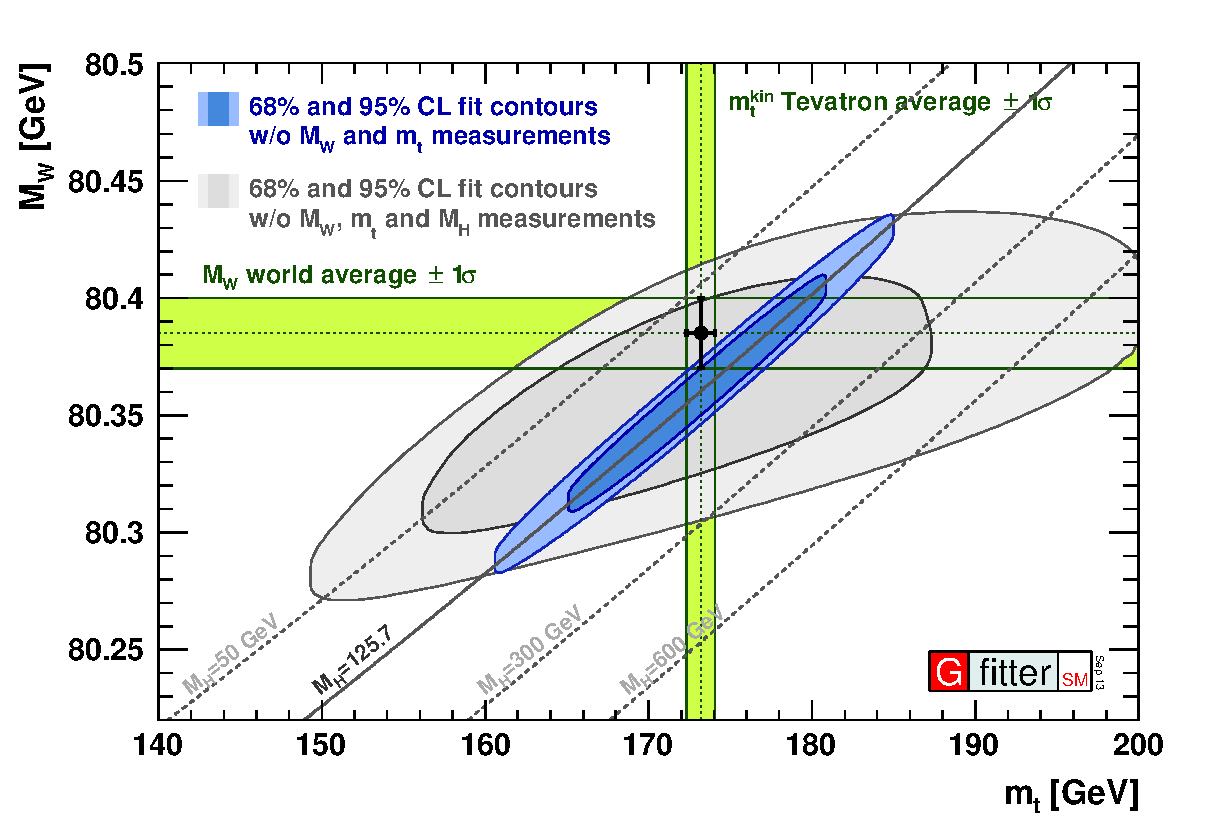
\includegraphics[width=0.8\textwidth]{pics/W_vs_top}


\end{minipage}\begin{minipage}{.45\textwidth}\centering

\vskip-5ex
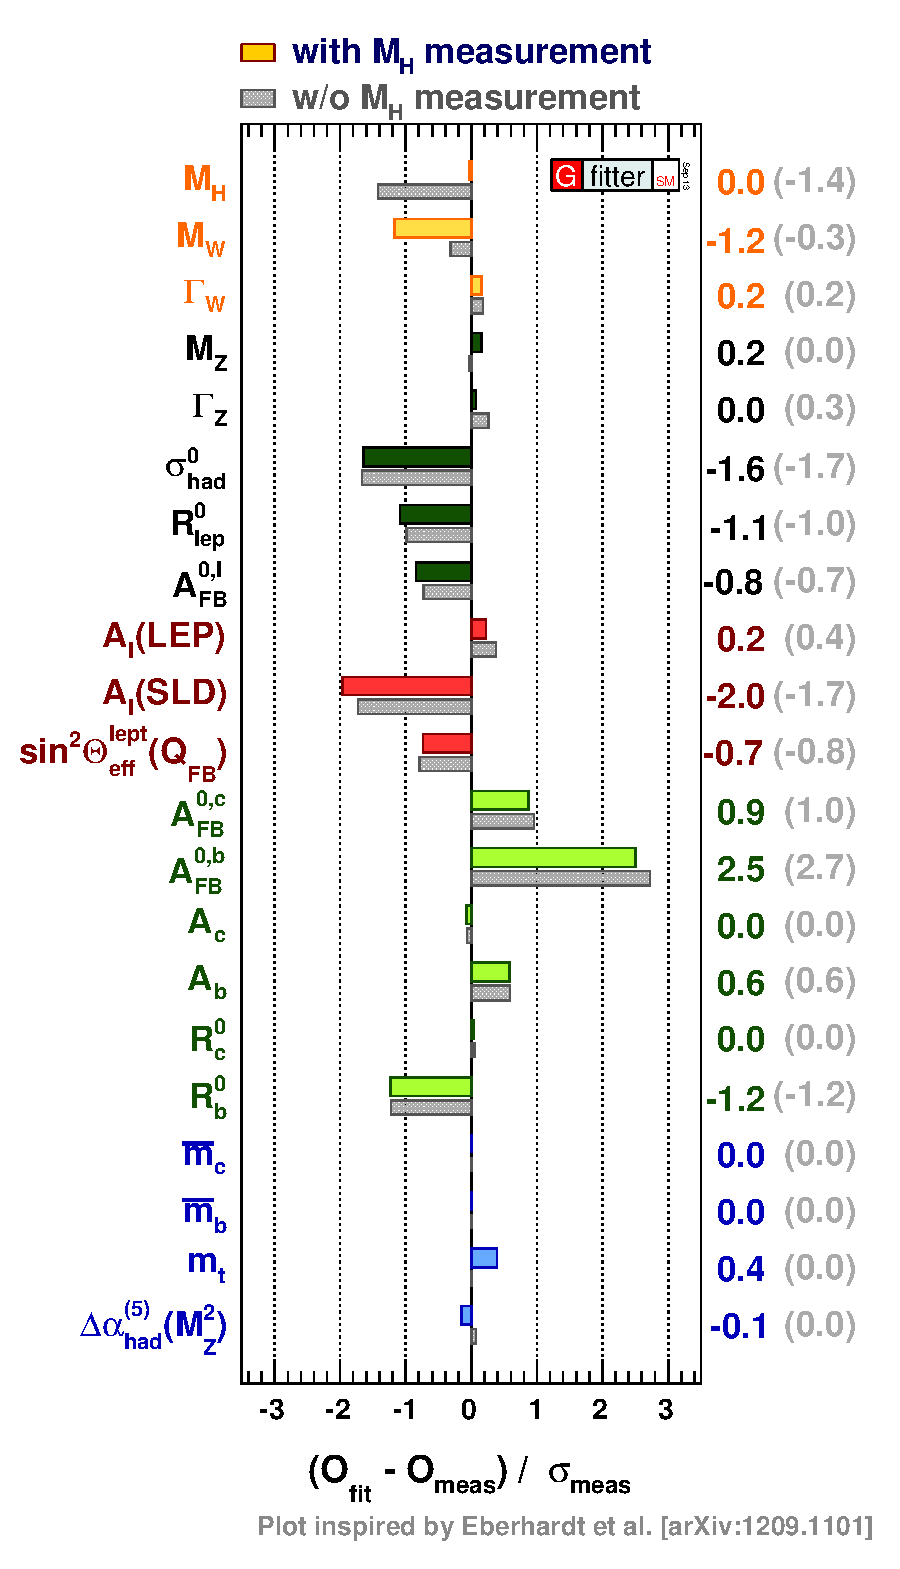
\includegraphics[width=0.8\textwidth]{pics/fitSM_new}

\end{minipage}\end{frame}


\begin{frame}\frametitle{\dots effectively}
\scriptsize\centering

\begin{pgfpicture}{0.0\textwidth}{0.0\textheight}{1.\textwidth}{.6\textwidth}

\begin{pgfscope}
\pgfdeclareimage[interpolate=true,width=.4\textwidth]{pie}{pics/piematter}
\pgfdeclareimage[interpolate=true,width=.42\textwidth]{gut}{pics/gut}
\pgfdeclareimage[interpolate=true,width=.3\textwidth]{loop}{pics/loop1}
\onslide<1->{
\pgfputat{\pgfxy(0.5,0.1)}{\pgfbox[left,base]{\pgfuseimage{gut}}}
\pgfputat{\pgfxy(3.,2.1)}{\pgfbox[left,base]{\small \bf\cccolor GUT theories? Gravity?}}
\pgfputat{\pgfxy(7.,3.6)}{\pgfbox[left,base]{\pgfuseimage{pie}}}
}
\onslide<2->{
   \begin{pgftranslate}{\pgfpoint{0.\textwidth}{0.\textheight}}
%%%%%%%% QUARKS
{\usebeamercolor[bg]{head/foot boxes}\pgfcircle[fill]{\pgfxy(1.0,6.5)}{10pt}}
\pgfputat{\pgfxy(0.85,6.4)}{\pgfbox[left,base]{\large$u$}}
{\usebeamercolor[bg]{head/foot boxes}\pgfcircle[fill]{\pgfxy(2.0,6.5)}{10pt}}
\pgfputat{\pgfxy(1.85,6.4)}{\pgfbox[left,base]{\large$c$}}
{\usebeamercolor[bg]{head/foot boxes}\pgfcircle[fill]{\pgfxy(3.0,6.5)}{10pt}}
\pgfputat{\pgfxy(2.85,6.4)}{\pgfbox[left,base]{\large$t$}}
{\usebeamercolor[bg]{head/foot boxes}\pgfcircle[fill]{\pgfxy(1.0,5.5)}{10pt}}
\pgfputat{\pgfxy(0.85,5.4)}{\pgfbox[left,base]{\large$d$}}
{\usebeamercolor[bg]{head/foot boxes}\pgfcircle[fill]{\pgfxy(2.0,5.5)}{10pt}}
\pgfputat{\pgfxy(1.85,5.4)}{\pgfbox[left,base]{\large$s$}}
{\usebeamercolor[bg]{head/foot boxes}\pgfcircle[fill]{\pgfxy(3.0,5.5)}{10pt}}
\pgfputat{\pgfxy(2.85,5.4)}{\pgfbox[left,base]{\large$b$}}
%%%%%%%%%%% LEPTONS
{\usebeamercolor[bg]{head/foot boxes}\pgfcircle[fill]{\pgfxy(1.0,4.5)}{10pt}}
\pgfputat{\pgfxy(0.85,4.4)}{\pgfbox[left,base]{\large$e$}}
{\usebeamercolor[bg]{head/foot boxes}\pgfcircle[fill]{\pgfxy(2.0,4.5)}{10pt}}
\pgfputat{\pgfxy(1.85,4.4)}{\pgfbox[left,base]{\large$\mu$}}
{\usebeamercolor[bg]{head/foot boxes}\pgfcircle[fill]{\pgfxy(3.0,4.5)}{10pt}}
\pgfputat{\pgfxy(2.85,4.4)}{\pgfbox[left,base]{\large$\tau$}}
{\usebeamercolor[bg]{head/foot boxes}\pgfcircle[fill]{\pgfxy(1.0,3.5)}{10pt}}
\pgfputat{\pgfxy(0.85,3.4)}{\pgfbox[left,base]{\large$\nu_{e}$}}
{\usebeamercolor[bg]{head/foot boxes}\pgfcircle[fill]{\pgfxy(2.0,3.5)}{10pt}}
\pgfputat{\pgfxy(1.85,3.4)}{\pgfbox[left,base]{\large$\nu_{\mu}$}}
{\usebeamercolor[bg]{head/foot boxes}\pgfcircle[fill]{\pgfxy(3.0,3.5)}{10pt}}
\pgfputat{\pgfxy(2.85,3.4)}{\pgfbox[left,base]{\large$\nu_{\tau}$}}

\pgfputat{\pgfxy(0.5,7.0)}{\pgfbox[left,base]{\small\bf \textit{the ``flavor puzzle''}}}
%%%%%%%%%%%% WHY
{ \pgfsetlinewidth{1.pt}
  \usebeamercolor[fg]{head/foot boxes}
  \pgfrect[stroke]{\pgfxy(3.6,3.)}{\pgfxy(2.7,4)}
  \usebeamercolor[fg]{normal text}
  \pgfputat{\pgfxy(3.5,5.)}{\pgfbox[left,base]{\footnotesize\begin{tabular}{c} why three\\ generations?\\ \\mass hierarchy?\\ \\baryon-antibaryon\\asymmetry?\end{tabular}}}
  %\pgfputat{\pgfxy(3.5,5.)}{\pgfbox[left,base]{\footnotesize\begin{tabular}{c} why only\\ 3 generations?\\ \\QCD limit:\\ 9 families\\ EW precision:\\ 3 neutrinos\\w/ $m_{\nu\nu}<m_Z$\\ \\baryon-antibaryon\\asymmetry?\end{tabular}}}
}
   \end{pgftranslate}
}
\onslide<3->{
   \begin{pgftranslate}{\pgfpoint{0.5\textwidth}{0.05\textheight}}
\pgfputat{\pgfxy(1.5,0.1)}{\pgfbox[left,base]{\pgfuseimage{loop}}}
\pgfputat{\pgfxy(1.7,2.1)}{\pgfbox[left,base]{\small\bf \textit{hierarchy problem}}}
\pgfputat{\pgfxy(1.7,0.4)}{\pgfbox[left,base]{\small $H \qquad\qquad t \qquad\qquad H$ }}
   \end{pgftranslate}
}

\end{pgfscope}
\end{pgfpicture}



\end{frame}


\begin{frame}\frametitle{Go Beyond!}
\scriptsize\centering

\begin{pgfpicture}{0.0\textwidth}{0.0\textheight}{1.\textwidth}{.6\textwidth}

\begin{pgfscope}
%\pgfdeclareimage[interpolate=true,width=.28\textwidth]{kk}{pics/extradimension.pdf}
\pgfdeclareimage[interpolate=true,width=.25\textwidth]{kk}{pics/extradimension.pdf}
\pgfdeclareimage[interpolate=true,width=.38\textwidth]{ed}{../theory/figures/I15-71-warpedi.jpg}
\pgfdeclareimage[interpolate=true,width=.6\textwidth]{compo}{../theory/figures/compHiggs.png}
\pgfdeclareimage[interpolate=true,width=.45\textwidth]{susy}{pics/susy}
\onslide<1->{
   \begin{pgftranslate}{\pgfpoint{0.0\textwidth}{0.\textheight}}
     %%%%%%%% QUARKS
{\usebeamercolor[bg]{head/foot boxes}\pgfcircle[fill]{\pgfxy(1.0,6.5)}{10pt}}
\pgfputat{\pgfxy(0.85,6.4)}{\pgfbox[left,base]{\large$u$}}
{\usebeamercolor[bg]{head/foot boxes}\pgfcircle[fill]{\pgfxy(2.0,6.5)}{10pt}}
\pgfputat{\pgfxy(1.85,6.4)}{\pgfbox[left,base]{\large$c$}}
{\usebeamercolor[bg]{head/foot boxes}\pgfcircle[fill]{\pgfxy(3.0,6.5)}{10pt}}
\pgfputat{\pgfxy(2.85,6.4)}{\pgfbox[left,base]{\large$t$}}
{\usebeamercolor[bg]{head/foot boxes}\pgfcircle[fill]{\pgfxy(1.0,5.5)}{10pt}}
\pgfputat{\pgfxy(0.85,5.4)}{\pgfbox[left,base]{\large$d$}}
{\usebeamercolor[bg]{head/foot boxes}\pgfcircle[fill]{\pgfxy(2.0,5.5)}{10pt}}
\pgfputat{\pgfxy(1.85,5.4)}{\pgfbox[left,base]{\large$s$}}
{\usebeamercolor[bg]{head/foot boxes}\pgfcircle[fill]{\pgfxy(3.0,5.5)}{10pt}}
\pgfputat{\pgfxy(2.85,5.4)}{\pgfbox[left,base]{\large$b$}}
%%%%%%%%%%% LEPTONS
{\usebeamercolor[bg]{head/foot boxes}\pgfcircle[fill]{\pgfxy(1.0,4.5)}{10pt}}
\pgfputat{\pgfxy(0.85,4.4)}{\pgfbox[left,base]{\large$e$}}
{\usebeamercolor[bg]{head/foot boxes}\pgfcircle[fill]{\pgfxy(2.0,4.5)}{10pt}}
\pgfputat{\pgfxy(1.85,4.4)}{\pgfbox[left,base]{\large$\mu$}}
{\usebeamercolor[bg]{head/foot boxes}\pgfcircle[fill]{\pgfxy(3.0,4.5)}{10pt}}
\pgfputat{\pgfxy(2.85,4.4)}{\pgfbox[left,base]{\large$\tau$}}
{\usebeamercolor[bg]{head/foot boxes}\pgfcircle[fill]{\pgfxy(1.0,3.5)}{10pt}}
\pgfputat{\pgfxy(0.85,3.4)}{\pgfbox[left,base]{\large$\nu_{e}$}}
{\usebeamercolor[bg]{head/foot boxes}\pgfcircle[fill]{\pgfxy(2.0,3.5)}{10pt}}
\pgfputat{\pgfxy(1.85,3.4)}{\pgfbox[left,base]{\large$\nu_{\mu}$}}
{\usebeamercolor[bg]{head/foot boxes}\pgfcircle[fill]{\pgfxy(3.0,3.5)}{10pt}}
\pgfputat{\pgfxy(2.85,3.4)}{\pgfbox[left,base]{\large$\nu_{\tau}$}}

{\usebeamercolor[bg]{head/foot boxes}\pgfcircle[fill]{\pgfxy(4.0,6.5)}{10pt}}
\pgfputat{\pgfxy(3.85,6.4)}{\pgfbox[left,base]{\large$t'$}}
{\usebeamercolor[bg]{head/foot boxes}\pgfcircle[fill]{\pgfxy(4.0,5.5)}{10pt}}
\pgfputat{\pgfxy(3.85,5.4)}{\pgfbox[left,base]{\large$b'$}}
%%%%%%%%%%% LEPTONS
{\usebeamercolor[bg]{head/foot boxes}\pgfcircle[fill]{\pgfxy(4.0,4.5)}{10pt}}
\pgfputat{\pgfxy(3.85,4.4)}{\pgfbox[left,base]{\large$\tau'$}}
{\usebeamercolor[bg]{head/foot boxes}\pgfcircle[fill]{\pgfxy(4.0,3.5)}{10pt}}
\pgfputat{\pgfxy(3.85,3.4)}{\pgfbox[left,base]{\large$\nu_{\tau'}$}}

     \pgfputat{\pgfxy(-0.1,5.)}{\pgfbox[left,base]{\small \cccolor \bf SM4}}
{ \pgfsetlinewidth{1.pt}
  \usebeamercolor[fg]{head/foot boxes}
     \pgfrect[stroke]{\pgfxy(3.5,3.)}{\pgfxy(1.,4)}
}
   \end{pgftranslate}
}
\onslide<2->{
%\pgfputat{\pgfxy(8.3,5.)}{\pgfbox[left,base]{\pgfuseimage{ed}}}
%\pgfputat{\pgfxy(8.3,0.)}{\pgfbox[left,base]{\pgfuseimage{kk}}}
\pgfputat{\pgfxy(4.55,1.8)}{\pgfbox[left,base]{\pgfuseimage{ed}}}
\pgfputat{\pgfxy(9.3,0.3)}{\pgfbox[left,base]{\pgfuseimage{kk}}}
}
\onslide<3->{
\pgfputat{\pgfxy(0.2,-0.1)}{\pgfbox[left,base]{\pgfuseimage{compo}}}
\pgfputat{\pgfxy(1.,2.1)}{\pgfbox[left,base]{\small \cccolor Composite Higgs}}
%\pgfputat{\pgfxy(3.,2.1)}{\pgfbox[left,base]{\small \cccolor Composite Higgs}}
}
\onslide<4->{
\pgfputat{\pgfxy(6.9,5.7)}{\pgfbox[left,base]{\pgfuseimage{susy}}}
}
\onslide<5->{
%\pgfputat{\pgfxy(5.3,4.8)}{\pgfbox[left,base]{\large \begin{tabular}{|c|} \toprule All\\ featuring\\ \bf \cccolor heavy\\ 
\pgfputat{\pgfxy(4.9,6.8)}{\pgfbox[left,base]{\normalsize \begin{tabular}{|c|} \toprule All\\ featuring\\ \bf \cccolor heavy\\ 
\bf \cccolor top\\ 
\bf \cccolor partner\\\bottomrule \end{tabular}}}
}



\end{pgfscope}
\end{pgfpicture}

\end{frame}


\begin{frame}\frametitle{Heavy quark production}
\centering

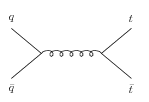
\includegraphics[width=0.2\textwidth]{../theory/figures/toppairprod/qqbdiag}
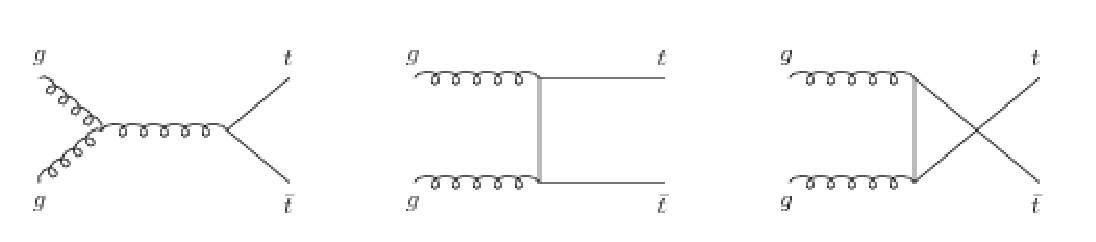
\includegraphics[width=0.65\textwidth]{../theory/figures/toppairprod/ggdiag}

\myskip

\begin{minipage}{.5\textwidth}\centering
\scriptsize

{\cccolor \bf Pair production} analogous to \ttbar:\\
$gg,q \bar q \to Q \bar Q \quad\quad (Q=T,B,X,Y)$\\
{\large$\Downarrow$}\\
``universal'': depends only on \alphas\ and $m_Q$\\

\myskip

\includegraphics[width=0.7\textwidth]{pics/singleprod}

\myskip

{\cccolor \bf Single production}:\\
$q q' \xrightarrow{V*} q_1Q \quad\quad (V=W,Z)$\\
{\large$\Downarrow$}\\
depends on couplings with $W$ and $Z$ bosons~\cite{Aguilar-Saavedra:2013qpa,Atre:2011ae}

\end{minipage}\begin{minipage}{.5\textwidth}\centering

\begin{pgfpicture}{0.0\textwidth}{0.0\textheight}{1.\textwidth}{.6\textwidth}
\pgfdeclareimage[interpolate=true,width=.9\textwidth]{xsec8}{pics/ja/fig4a}
\pgfputat{\pgfxy(0.1,0.)}{\pgfbox[left,base]{\pgfuseimage{xsec8}}}
 {
   \pgfsetlinewidth{1.5pt}
   \usebeamercolor[fg]{head/foot boxes}
   \pgfline{\pgfxy(2.68,0.4)}{\pgfxy(2.68,2.9)}
 }
\end{pgfpicture}
\end{minipage}

\end{frame}


\begin{frame}\frametitle{Decay modes and available signatures}
\centering
\scriptsize

\begin{minipage}{.65\textwidth}\centering
\begin{itemize}
\item Chiral $t'\to Wb$ 100\% (comes in $SU(2)$ doublet)
\item Vector-like $T(+2/3)$, $B(-1/3)$, $X(+5/3)$, $Y(-4/3)$ 
\end{itemize}
$L$ and $R$ components transform the same under $SU(2)$\\
Decay modes depending on {\it quantum numbers}\\ 
Assume mixing mainly with 3$^{\rm rd}$ generation SM quarks

\myskip

  \begin{tabular}{ccccccc}\toprule
%Singlet & Decay modes\\ 
          &                    & 4$l$ & 3$l$ & 2$l$ & 2$l$ & 1$l$ +\\
          &                    &      &      & OS   & SS   & jets \\
$T(+2/3)$ & $W^+b,\, Ht,\, Zt$ & \large\checkmark &\large\checkmark &\large\checkmark & &\large\checkmark\\
& \\
$B(-1/3)$ & $ W^-t,\, Hb,\, Zb$ & \large\checkmark &\large\checkmark &\large\checkmark &\large\checkmark &\large\checkmark \\
%& \\\midrule
%Doublet & Decay modes\\
 &\\
 \multirow{2}{*}{$\bigg(\begin{array}{c}T \\ B\end{array}\bigg)$} & $W^+b,\, Ht,\, Zt$  & \large\checkmark &\large\checkmark &\large\checkmark & &\large\checkmark\\
 & $ W^-t,\, Hb,\, Zb$ & \large\checkmark &\large\checkmark &\large\checkmark &\large\checkmark &\large\checkmark\\
 & \\
\multirow{2}{*}{$\bigg(\begin{array}{c}T \\ X\end{array}\bigg)$} & $Ht,\, Zt$ & \large\checkmark &\large\checkmark &\large\checkmark & &\large\checkmark\\
 & $W^+t$ & \large\checkmark &\large\checkmark &\large\checkmark &\large\checkmark &\large\checkmark\\
 &\\
 \multirow{2}{*}{$\bigg(\begin{array}{c}B \\ Y\end{array}\bigg)$} & $Hb,\, Zb$ & \large\checkmark & & \large\checkmark & & \\
 & $W^-b$ &  & &\large\checkmark & &\large\checkmark\\
\bottomrule
\end{tabular}


\end{minipage}

\end{frame}

